\chapter{Thiết kế và Cài đặt}

\section{Kiến trúc tổng thể của hệ thống}

Hệ thống được thiết kế theo mô hình client–server với hai thành phần chính:

\begin{itemize}
  \item \textbf{Client}: thực hiện nén tệp, mã hóa và gửi dữ liệu.
  \item \textbf{Server}: nhận dữ liệu, giải mã và giải nén để khôi phục tệp gốc.
\end{itemize}

Quá trình truyền dữ liệu đảm bảo tính bảo mật và toàn vẹn nhờ áp dụng kết hợp kỹ thuật mã hóa đối xứng và nén tệp. Hình \ref{fig:system_architecture} minh họa kiến trúc tổng thể của hệ thống.

\begin{figure}[H]
  \centering
  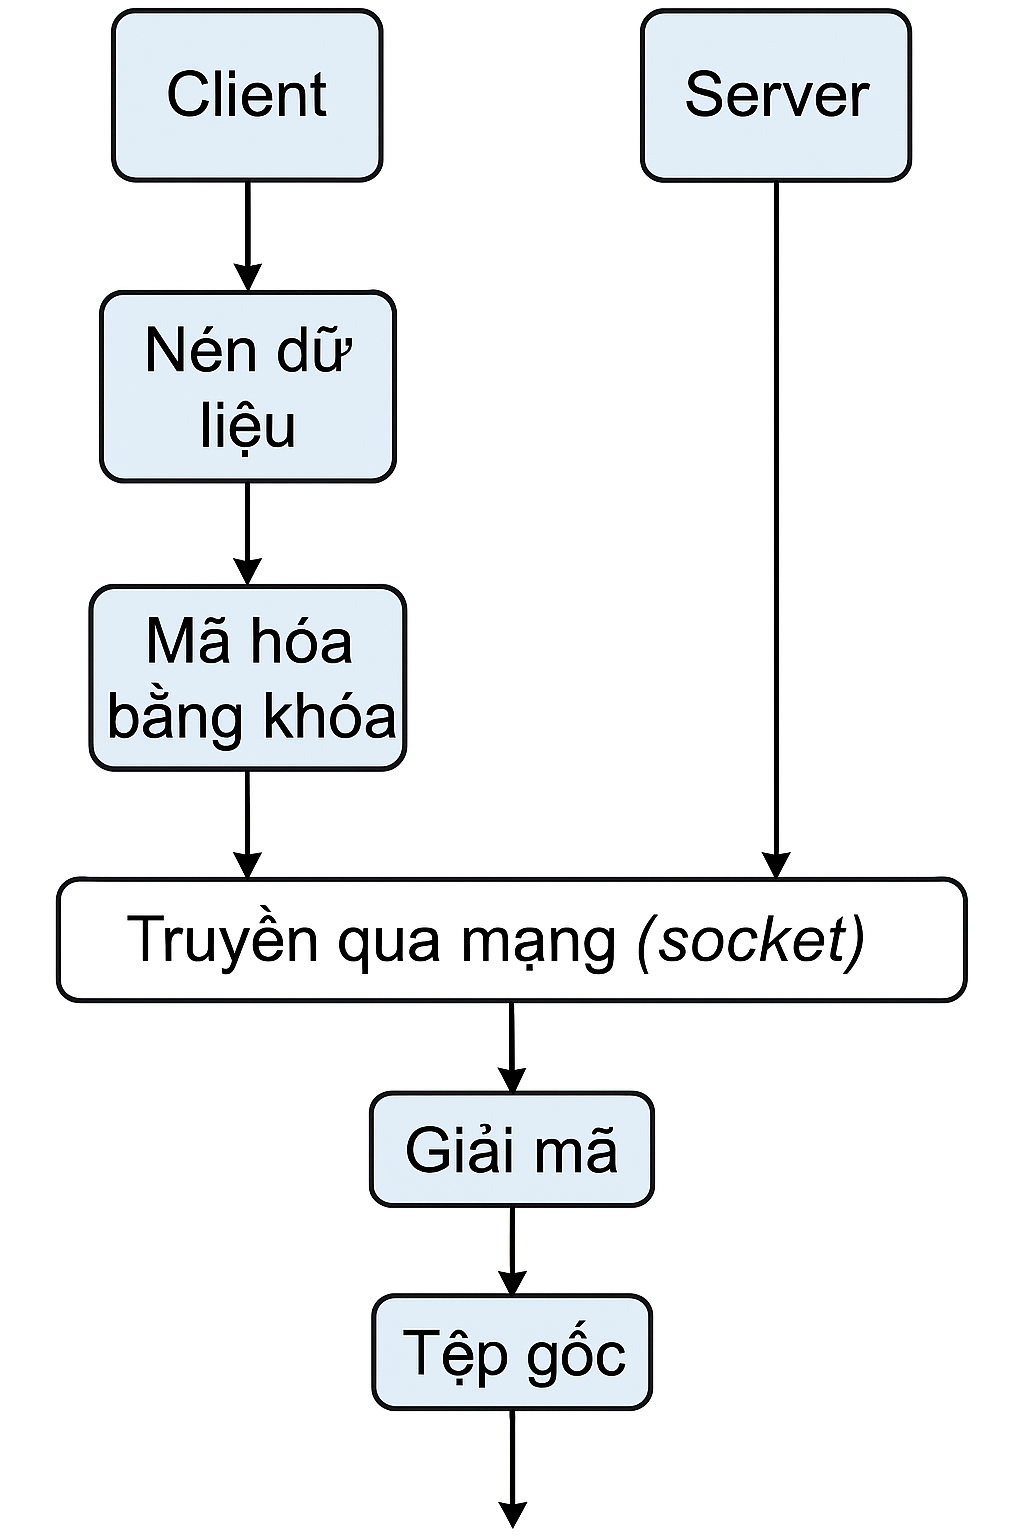
\includegraphics[width=0.95\textwidth]{figs/architecture.png}
  \caption{Kiến trúc hệ thống gửi báo cáo tài chính}
  \label{fig:system_architecture}
\end{figure}

\section{Quy trình xử lý tại phía Client}

Các bước xử lý tại máy khách bao gồm:

\begin{enumerate}
  \item Chọn tệp đầu vào (ví dụ: \texttt{financial\_report.pdf}).
  \item Nén tệp bằng thư viện \texttt{zipfile}, tạo ra tệp \texttt{compressed.zip}.
  \item Mã hóa tệp nén sử dụng thuật toán đối xứng (Fernet – AES 128-bit).
  \item Gửi dữ liệu đã mã hóa qua socket TCP tới địa chỉ IP của server.
\end{enumerate}

Client có thể được chạy từ dòng lệnh với các tham số như tên file, IP server, cổng kết nối.

\section{Quy trình xử lý tại phía Server}

Phía máy chủ thực hiện các bước sau:

\begin{enumerate}
  \item Mở socket TCP và lắng nghe kết nối từ client.
  \item Nhận dữ liệu mã hóa từ client và lưu vào tệp \texttt{received\_encrypted.bin}.
  \item Giải mã dữ liệu bằng khóa bí mật đã chia sẻ.
  \item Giải nén tệp để khôi phục nội dung ban đầu (PDF).
\end{enumerate}

Sau khi hoàn tất, báo cáo tài chính gốc sẽ được lưu vào thư mục đích để kiểm tra.

\begin{algorithm}[H]
\caption{Tổng quan quy trình xử lý dữ liệu tại Client và Server}
\begin{algorithmic}[1]
\State \textbf{Client:}
\State Chọn tệp $\rightarrow$ Nén bằng ZIP $\rightarrow$ Mã hóa bằng Fernet
\State Gửi dữ liệu đã mã hóa đến server qua socket
\Statex
\State \textbf{Server:}
\State Lắng nghe socket $\rightarrow$ Nhận file $\rightarrow$ Giải mã $\rightarrow$ Giải nén
\end{algorithmic}
\end{algorithm}


\section{Chi tiết mã nguồn}

Toàn bộ mã nguồn được chia thành các module Python rõ ràng, gồm:

\begin{itemize}
  \item \textbf{client.py}: xử lý nén, mã hóa và gửi dữ liệu.
  \item \textbf{server.py}: lắng nghe kết nối, nhận và xử lý dữ liệu.
  \item \textbf{utils.py}: chứa các hàm dùng chung như tạo khóa, mã hóa/giải mã.
\end{itemize}

Một đoạn mã minh họa quá trình nén và mã hóa như sau:

\begin{lstlisting}[language=Python, caption={Hàm nén và mã hóa tệp tại client}, label={code:encrypt}]
def compress_and_encrypt(file_path, key):
    zip_path = file_path + ".zip"
    with zipfile.ZipFile(zip_path, 'w') as zipf:
        zipf.write(file_path, os.path.basename(file_path))
    with open(zip_path, 'rb') as f:
        data = f.read()
    fernet = Fernet(key)
    encrypted = fernet.encrypt(data)
    return encrypted
\end{lstlisting}

\section{Yêu cầu hệ thống}

Để chạy hệ thống, máy tính cần cài đặt:

\begin{itemize}
  \item Python 3.10 trở lên
  \item Thư viện: \texttt{cryptography}, \texttt{zipfile}, \texttt{socket}
  \item Kết nối mạng TCP nội bộ (LAN) hoặc mô phỏng qua localhost
\end{itemize}

Tất cả các thành phần được cài đặt đơn giản bằng pip và chạy trực tiếp qua dòng lệnh.

